\section{Demystifying the EEG System Framework}
\label{sec:framework}

Before proceeding to introduce our new attack vectors, we first investigated the system framework adopted by the NeuroSky devices. As we mentioned in Section~\ref{sec:background}, most NeuroSky devices leverage TGAM, which employs the EEG system framework. Unfortunately, NeuroSky does not explicitly publicize the specification details of the framework; therefore we conducted an empirical study by both reading the related documents such as the development guide and user guide published publicly, and conducting dynamic testing cases, to thoroughly recover the EEG system framework. We found that the EEG system framework can be separated into two sides, the user application side where high-level BCI apps reside and the headset side where brain waves are collected and transmitted. 

\subsection{User Application Side}
In the EEG system framework, the software-level implementations and operations are all integrated on the user's application side, whose hardware devices include the user's PC where BCI apps are running on and a radio frequency (RF) dongle serving as a communication bridge between BCI apps and the EEG headset, which is attached to the PC via a USB port. After exploring the developer's documentation, we recovered the sub-framework on the user application side and found that a BCI app running on the user's PC has the following two ways of retrieving the brain wave data: either from the standard software development kit (SDK) which retrieves the requested data from the RF dongle through the USB serial port, or via a pre-defined low-level socket protocol called ThinkGear socket protocol (TGSP). 

\subsubsection{EEG Data Retrieval through Standard SDK}
The EEG system framework provides a standard SDK for Windows operating systems so that Windows-based BCI apps can directly invoke API calls provided by the SDK for EEG data retrieval and all the necessary API functions are offered by a dynamic link library (DLL) binary file called \texttt{thinkgear.dll}. Unfortunately, the documentation lacks a systematic demonstration of the APIs in the DLL; therefore we reversely engineered the DLL and found that besides the DLL main entry function \texttt{DLLEntryPoint}, it exports 19 other API functions. After a further exploration, we identified 4 functions that are mandatory to complete an EEG data retrieval; the other 15 functions are optional as they perform tasks such as writing a log stream, setting a baud rate, and reading a driver's version. The 4 mandatory functions are \texttt{TG\_GetNewConnectionId} through which the API caller is assigned an available integer as an identifier for a new connection to the RF dongle serial port, \texttt{TG\_Connect} which initializes a new connection that is bound with the provided connection id, \texttt{TG\_ReadPackets} which reads a raw packet through the RF dongle serial port, and \texttt{TG\_GetValue} which parses and returns a requested EEG data from a raw packet. The calls have to be made in the order of \texttt{TG\_GetNewConnectionId}, \texttt{TG\_Connect}, \texttt{TG\_ReadPackets}, and finally \texttt{TG\_GetValue}.

\subsubsection{EEG Data Retrieval through TGSP}
The EEG system framework also provides a low-level socket protocol, TGSP, for EEG data retrieval. TGSP can not only simplify the EEG data retrieval process since BCI apps do not need to go through the tedious SDK API calls, but also allow BCI apps to be implemented on different platforms other than Windows. TGSP adopts a server-client structure where there is an official server provided by NeuroSky, called ThinkGear Connector (TGC), which runs on the user's Windows platform, and BCI apps serve as clients sending requests to TGC and retrieving the desired data. \\
%
\indent The communications between TGC and the RF dongle is not complicated. As a matter of fact, the method leveraged by TGC to retrieve the EEG data from the RF dongle is fundamentally identical to the standard SDK; however, TGC integrates the API functions inside the TGC program with Windows .NET framework instead of making API calls to \texttt{thinkgear.dll}. The communications between TGC and BCI apps follow the following procedure: TGC first opens a fixed TCP port number \texttt{13854}, then a BCI app verifies itself with the TGC by sending a JSON request with the format shown below:
\begin{lstlisting}[language=json]
{"appName": "some app name", "appKey":"some app key"}
\end{lstlisting}
where the attribute \texttt{appName} is the name of the BCI app and \texttt{appKey} is a SHA-1 key of \texttt{appName} according to the documentation. Normally, the \texttt{appKey} should serve as a verification code for authentication. However, after a further exploration we noticed that the \texttt{appKey} serves merely as the app's identifier instead of a secret key assigned by the server; therefore, the whole verification process has little security implication. \\
%
\indent After the verification process, the BCI app can send a request with the following format to retrieve the EEG data from TGC:
\begin{lstlisting}[language=json]
{"enableRawOutput": true/false, "format": "Json/BinaryPacket"}
\end{lstlisting}
where \texttt{enableRawOutput} indicates whether or not TGC should return the raw voltage data from the three electrodes and \texttt{format} specifies whether TGC should return the data in the format of JSON or as a binary raw packet. \\
%
\indent If requested with the JSON format, TGC responds with the format shown below:
\begin{lstlisting}[language=json]
{"poorSignalLevel":n1,"eSense":{"attention":n2,"meditation":n3},"eegPower":{"delta":n4,"theta":n5,"lowAlpha":n6,"highAlpha":n7,"lowBeta":n8,"highBeta":n9,"lowGamma":n10,"highGamma":n11}}
\end{lstlisting}
where \texttt{poorSignalLevel} specifies the poorness level (ranging from 0 to 200, with 0 indicating a good signal while 200 indicating the off-head state) of the signal resulted from how properly the user wears the headset.\\
%
\indent If requested with the \texttt{BinaryPacket} format, TGC responds with raw packets following the structure shown in Table~\ref{tbl:basicpacket}. A packet begins with two \texttt{SYNCS} of value \texttt{0xAA} for each, followed by one byte indicating the length of the payload, the payload itself, and the 1-byte checksum for the payload. The payload is stacked with a number of \texttt{DataRow}s. A  \texttt{DataRow} is a special structure shown in Table~\ref{tbl:datarow} with a size of PLENGTH ranging from 1 to 256 bytes. It begins with an optional segment called \texttt{EXCODE} valued \texttt{0x55} with undefined size (undefined number of \texttt{0x55}s), followed by the 1-byte \texttt{CODE} indicating what type of data is passed, an optional 1-byte segment \texttt{VLENGTH} indicating the length of the value, and finally the value itself. The choices of \texttt{CODE} values are documented in~\cite{tgsprawpacket}. Some of the most important ones include \texttt{0x02}, \texttt{0x04}, \texttt{0x05}, and \texttt{0x81}, representing poorness level of the signal, attention meter, meditation meter, and EEG power, respectively. 

%%%%%%%%% Basic Packet Structure
\begin{table}[]
\centering
\caption{TGSP Raw Packet Structure}
\label{tbl:basicpacket}
\scalebox{0.8}{
\begin{tabular}{llcccc}
\hline \hline
\multicolumn{2}{|r|}{SYNC}  & \multicolumn{1}{c|}{SYNC}     & \multicolumn{1}{c|}{PLENGTH}                                                      & \multicolumn{1}{c|}{PAYLOAD}                                                  & \multicolumn{1}{c|}{CHECKSUM}                                                                            \\ \hline \hline
\multicolumn{1}{|l|}{Content} & \multicolumn{1}{l|}{\texttt{0xAA}} & \multicolumn{1}{l|}{\texttt{0xAA}}  & \multicolumn{1}{c|}{\begin{tabular}[c]{@{}c@{}}Length of \\ payload\end{tabular}} & \multicolumn{1}{c|}{\begin{tabular}[c]{@{}c@{}}Series of\\ \texttt{DataRows}\end{tabular}} & \multicolumn{1}{c|}{\begin{tabular}[c]{@{}c@{}}Checks if the payload\\ has bit errors.\end{tabular}} \\ \hline
\multicolumn{1}{|l|}{Size}    & \multicolumn{1}{l|}{1 byte} & \multicolumn{1}{c|}{1 byte}                                                       & \multicolumn{1}{c|}{1 byte}                                                       & \multicolumn{1}{c|}{PLENGTH}                                                  & \multicolumn{1}{c|}{1 byte}                                                                              \\ \hline
                              &                             & \multicolumn{1}{l}{}                                                              & \multicolumn{1}{l}{}                                                          & \multicolumn{1}{l}{}                                                                                    
\end{tabular}
}
\end{table}

%%%%%% DataRow Structure
\begin{table}[]
\centering
\caption{Raw \texttt{DataRow} Structure}
\label{tbl:datarow}
\scalebox{0.8}{
\begin{tabular}{llccc}
\hline \hline
\multicolumn{2}{|r|}{(EXCODE)}                                  & \multicolumn{1}{c|}{CODE}                                                    & \multicolumn{1}{c|}{(VLENGTH)}                                                & \multicolumn{1}{c|}{VALUE}                                                       \\ \hline \hline
\multicolumn{1}{|l|}{Content} & \multicolumn{1}{l|}{\texttt{0x55}}       & \multicolumn{1}{c|}{\begin{tabular}[c]{@{}c@{}}Type of \\ data\end{tabular}} & \multicolumn{1}{c|}{\begin{tabular}[c]{@{}c@{}}Length of\\ Value\end{tabular}} & \multicolumn{1}{c|}{\begin{tabular}[c]{@{}c@{}}Value of\\ the data\end{tabular}} \\ \hline
\multicolumn{1}{|l|}{Size}    & \multicolumn{1}{l|}{Undefined} & \multicolumn{1}{c|}{1 byte}                                                  & \multicolumn{1}{c|}{1 byte}                                                   & \multicolumn{1}{c|}{VLENGTH}                                                  \\ \hline
                              &                                 & \multicolumn{1}{l}{}                                                         & \multicolumn{1}{l}{}                                                          & \multicolumn{1}{l}{}                                                            
\end{tabular}
}
\end{table}

\subsection{Headset Side}
In the EEG system framework, the TGAM chip in a headset collects user's EEG signals through the 3 electrodes and transmits the signals over-the-air through software defined radio (SDR). SDR is a novel radio technology in which the traditional components within the radio communication system such as mixers, filter, modulator, and demodulator, which are used to be implemented in hardware, are realized by software. In our case, the TGAM in the headset encodes the EEG raw packets into radio signals, applies one types of modulation to the signals, and finally propagates the signals at a certain range of frequency; while the RF dongle takes care of receiving the signal from the predetermined frequency, filtering noises, demodulating signals, and finally decoding the EEG raw packets. Even though the SDR specification is not included in the user manual guide provided by NeuroSky, fortunately, we found that the Federal Communication Commission (FCC) ID of the NeuroSky home-use EEG IoT device, ``XG9MW1'', is printed on the device headset. According to per U.S. law, all products which emit radio waves have to register with FCC to maintain test reports of radio specifications. After exploring the headset's test report~\cite{testreport} by searching the FCC ID, we found that the TGAM chip can operate on the frequency band ranging from $2419.9$ MHz to $2470.9$ MHz, and the modulation type is minimum shift keying (MSK) where messages are encoded into a sinusoid wave and a bit 0 and a bit 1 differ by half of a carrier period. %MSK has been widely adopted in industrial world for wireless communications; one of the most widely used MSK is called Gaussian minimum-shift keying (GMSK), which is a standard modulation method for GSM mobile phones.
\\
%
\indent However, as pointed out by the test report, a ThinkGear EEG device has an operable frequency range of $51$ MHz, which is too large for feasible analysis. In order to find the fine-grained center frequency via which the device is operating, we employed HackRF~\cite{gadgetshackrf}, a SDR peripheral device capable of transmitting and receiving radio signals from $1$ MHz to $6$ GHz, and GQRX~\cite{gqrx}, an open source SDR receiver powered by the GNU Radio. We conducted 30 experiments on 3 different NeuroSky EEG devices, 10 for each, and found that all devices in all experiments used the same center frequency with the same bandwidth: the approximate center frequency is $2458.4$ MHz with an occupied bandwidth of approximately $1$ MHz. A sample of the TGAM SDR wave is shown in Figure~\ref{fig:sdrsample}.\\
%
\indent According to our experimental study and analysis described above, we concluded that the entire EEG system framework can be sketched as in Figure~\ref{fig:tgframework}. It consists of four components: BCI apps, RF dongle, TGSP server, and TGAM. A BCI app is installed on the user's application side, and it has two ways of retrieving the user's EEG data when running, via either standard SDK or TGSP. If the BCI app requests an EEG data via the standard SDK, it directly communicates with the RF dongle through the USB serial port which returns the raw binary packet of the EEG data; if the BCI app requests an EEG data via the TGSP server (officially, the Thinkgear Connector), the server then retrieves the EEG data from the RF dongle likewise. Lastly, through SDR, the RF dongle receives the raw EEG data collected by the headset with the multi-modal sensor TGAM which employs three electrodes to measure the brain waves from a human scalp. The SDR has a center frequency roughly located at $2458.4$ MHz with an occupied bandwidth of approximately $1$ MHz.

\begin{figure}[!htb]
        \centering
        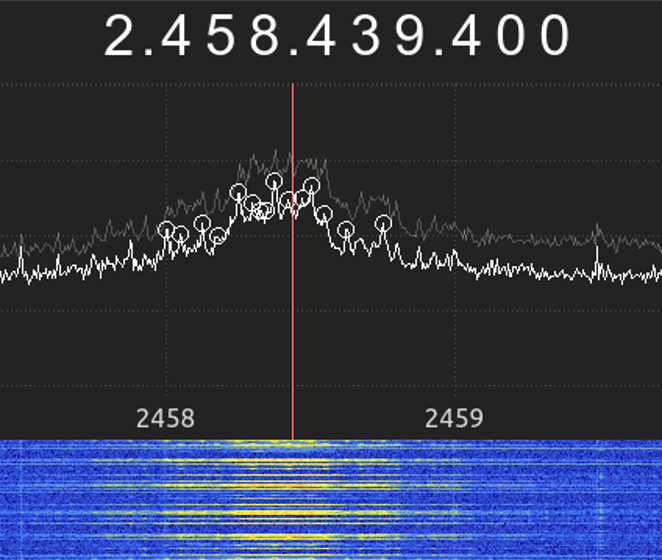
\includegraphics[scale=0.4]{sdr_sample.png}
        \caption{A sample of the TGAM SDR wave. The center frequency is roughly $2458.4$ MHz and the occupied bandwidth is approximately $1$ MHz.}
        \label{fig:sdrsample}
\end{figure}

\begin{figure}[!htb]
        \centering
        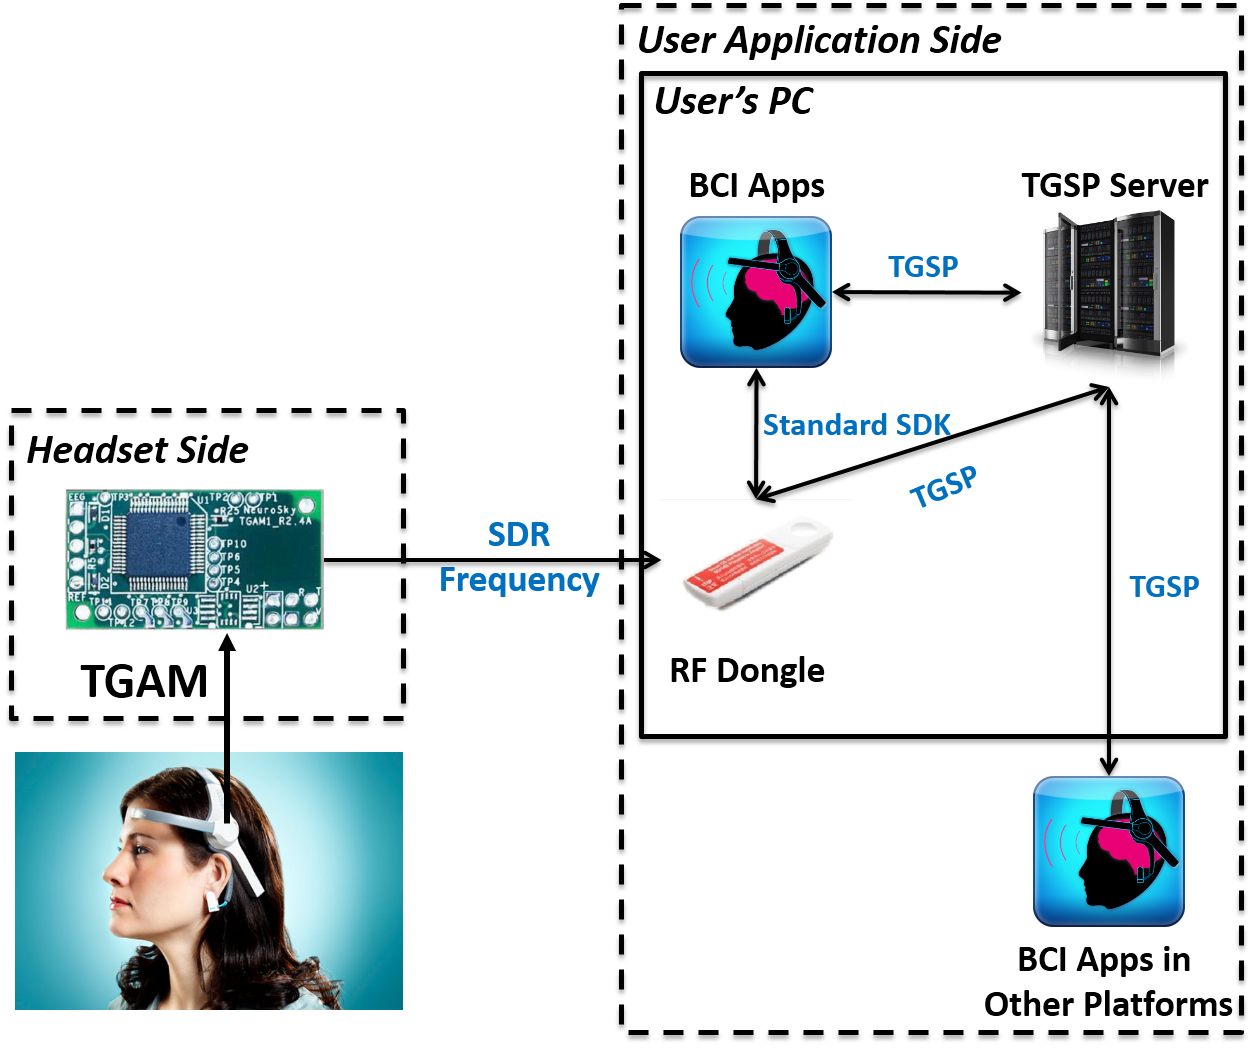
\includegraphics[scale=0.4]{tgframework.png}
        \caption{The diagram of the entire EEG system framework. A BCI app runs on a user's PC or other platforms within the user application side. If running on the user's PC, the BCI app can retrieve user's EEG data via either the standard SDK or TGSP. If running on a platform other than the user's PC, a BCI app can only retrieve the EEG data via TGSP. Both SDK and the TGSP server communicate with the RF dongle to retrieve the EEG data from the user's headset through a SDR network.}
        \label{fig:tgframework}
\end{figure}
